%\documentclass[preprint,tightenlines,showpacs,showkeys,floatfix,
%nofootinbib,superscriptaddress,fleqn]{revtex4} 
\documentclass[floatfix,nofootinbib,superscriptaddress,fleqn,preprint]{revtex4} 
%\documentclass[aps,epsfig,tightlines,fleqn]{revtex4}
\usepackage[utf]{kotex}
\usepackage[HWP]{dhucs-interword}
\usepackage[dvips]{color}
\usepackage{graphicx}
\usepackage{bm}
%\usepackage{fancyhdr}
%\usepackage{dcolumn}
\usepackage{defcolor}
\usepackage{amsmath}
\usepackage{amsfonts}
\usepackage{amssymb}
\usepackage{amscd}
\usepackage{amsthm}
\usepackage[utf8]{inputenc}
 \usepackage{setspace}
%\pagestyle{fancy}

\begin{document}

\title{\Large 2022년 1학기 물리학 I: Quiz 4}
\author{김현철\footnote{Office: 5S-436D (면담시간 매주
    화요일-16:00$\sim$20:00)}} 
\email{hchkim@inha.ac.kr}
\affiliation{Hadron Theory Group, Department of Physics, Inha University,
Incheon 402-751, Republic of Korea }
\date{Spring semester, 2022}


\vspace{1.cm}
\begin{abstract}
\noindent \textbf{ {\color{red}주의}: \color{blue} 단 한 번의 부정행위도 절대
  용납하지 않습니다. 적발 시, 학점은 F를 받게 됨은 물론이고,
  징계위원회에 회부합니다. One strike out임을 명심하세요.}\\
\\
문제는 다음 쪽부터 나옵니다.  \\ \\
{\bf Date:} 2022년 3월 14일 (월) 15:30--16:15
\\
{\bf 학번:} \hspace{4cm}
{\bf 이름:} 

\end{abstract}
\maketitle

\noindent {\bf 문제 1 [10pt]} 
그림~\ref{fig:1}과 같이 어떤 사람이 건물
꼭대기에서 수평에서부터 $30^\circ$의 각도로, 20.0 m/s의 속도로
공을 던졌다. 건물 
바닥에서 공을 던진 곳까지 높이는 45.0 m이다. 
\begin{figure}[ht]
  \centering
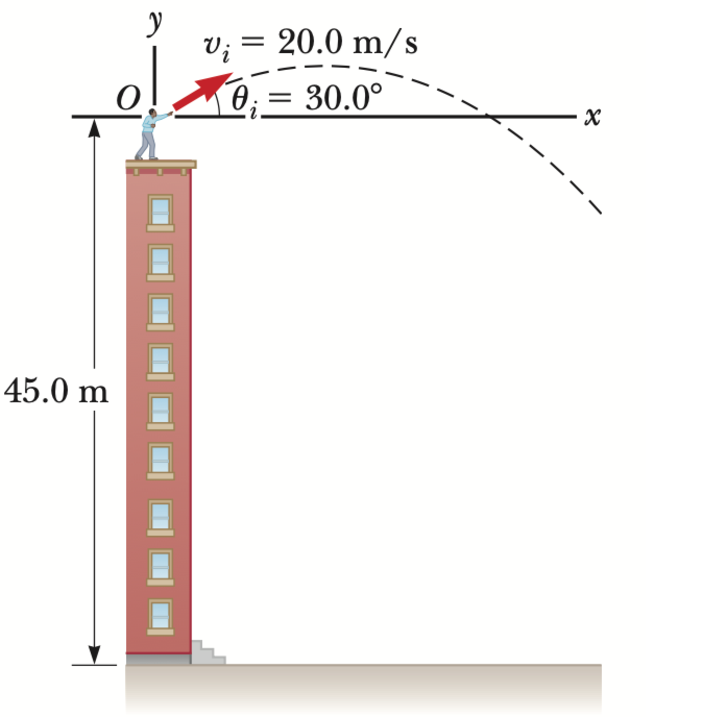
\includegraphics[scale=0.6]{Qfig4-2.pdf}  
  \caption{문제 2}
  \label{fig:1}
\end{figure}
\begin{itemize}
\item[(가)] 공이 지면에 닿을 때까지 걸린 시간을 구하여라.
\item[(나)] 공이 지면에 닿을 때 속력을 구하여라. (이 문제에서는 계산기를
  쓰셔도 무방합니다.)
\end{itemize}



\newpage

{\color{gray} [문제 풀이 쪽]}

\newpage 

\noindent {\bf 문제 2 [20pt]} 초기 위치 $x_0$, 초기 속력 $v_0$이
주어졌을 때, 아래의 식
\begin{align}
  \label{eq:1}
v^2 - v_0^2 = 2a(x-x_0)  
\end{align}
을 다음과 같이 유도해보자. 순간 가속도는
\begin{align}
  \label{eq:2}
a = \frac{dv}{dt}
\end{align}
와 같이 주어진다. \eqref{eq:2}의 양변에 속력 $v$를 곱한 식에서부터
\eqref{eq:1}을 유도하여라. (적분을 이용하여야 한다는 점을 명심하여라.)
\newpage

{\color{gray} [문제 풀이 쪽]}

\newpage 

\noindent {\bf 문제 3 [10pt]} 
스키 점프 선수가 트랙의 수평면에 도달해서
수평방향으로 도약을 했다. 이 때 속력은 20.0 m/s였다. 그리고 수평면과
경사면 사이의 각은 $35.0^\circ$였다. 이 선수는 어느 지점에 착지했을까? 
\begin{figure}[ht]
  \centering
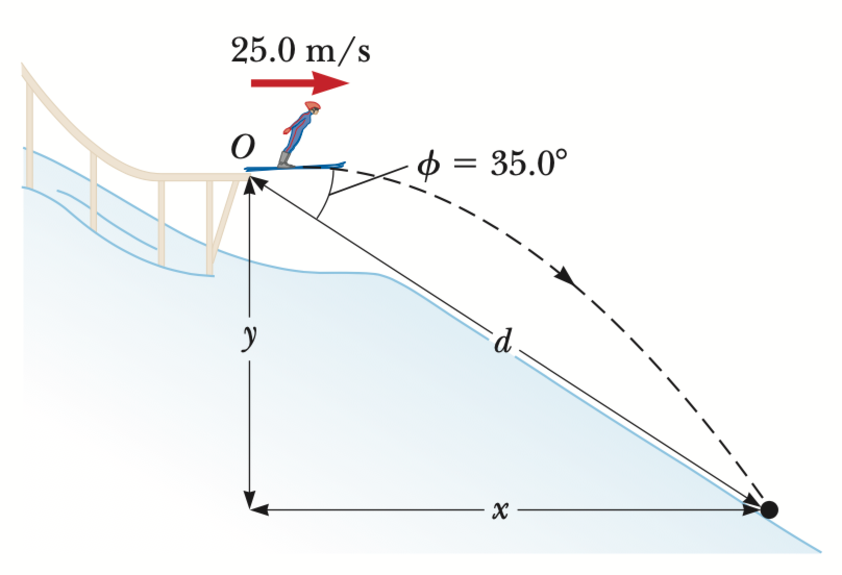
\includegraphics[scale=0.6]{Qfig4-3.pdf}  
  \caption{문제 3}
  \label{fig:2}
\end{figure}
\newpage

{\color{gray} [문제 풀이 쪽]}

\newpage

\noindent {\bf 문제 4 [10pt]} 높이가 $y_0=15.0$ m인 건물이 있다. 이 건물
꼭대기에서 $v_0=10.0$ m/s의 속력으로 위로 공을 쏘아올렸다. 
\begin{figure}[ht]
  \centering
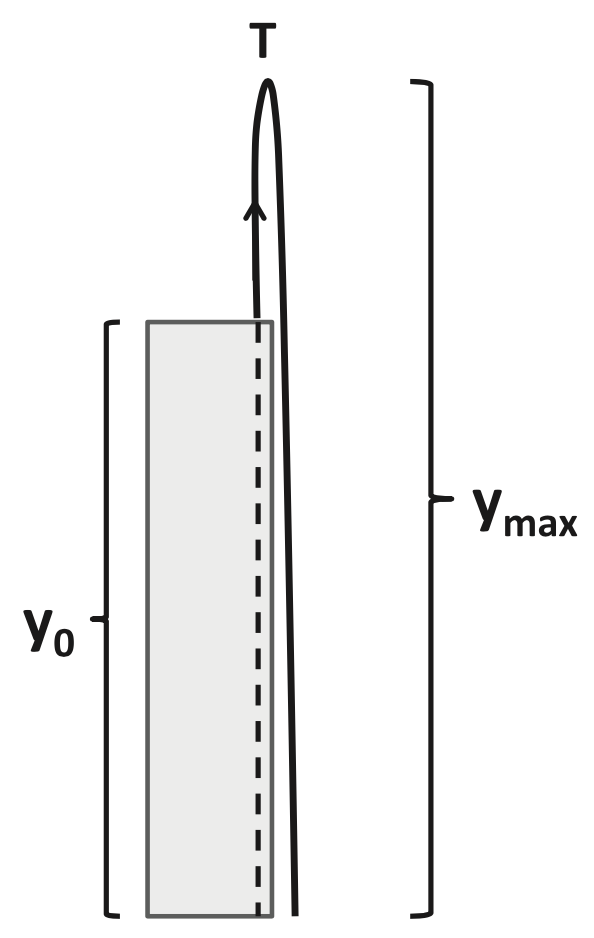
\includegraphics[scale=0.5]{Qfig4-4-20210312.png}  
  \caption{문제 4}
  \label{fig:4}
\end{figure}
그림~\ref{fig:4}에 보여주는 $y_{\mathrm{max}}$를 구하여라. 
\newpage

{\color{gray} [문제 풀이 쪽]}

\newpage
\end{document}